% Project Specifications

\chapter{Generator Layers}

\section{Transposed Convolutional Layer}

In CNNs, convolutional layer extracts various features from the input, essentially performing a downsampling
operation. Transposed convolutional layer, also known as fractionally strided convolutional layers, or sometime
erroneously as deconvolutional layer, on the other hand performs upsampling on the input. Normally unsampling
is often done with interpolation, but transposed convolution as a novel approach offers trainability which
makes it useful for neural networks. Conceptually, if we run a convolution of stride $f$ backwards,
it can be seen as convolution with stride $1/f$, hence the name fractionally strided convolution.

\subsection{Convolution}

To understand its operation, let us work though a simple numerical example. We begin with regular convolution
with an input of $4 \times 4$ matrix $A$:

$$
A =
  \begin{pmatrix}
    1 & 2 & 3 & 4 \\
    4 & 3 & 2 & 1 \\
    1 & 2 & 3 & 4 \\
    4 & 3 & 2 & 1
  \end{pmatrix}
$$

Let the kernel be a $2x2$ matrix $K$:

$$
K =
  \begin{pmatrix}
    1 & 2 \\
    3 & 4
  \end{pmatrix}
$$

Assume the convolution operates with padding of $1$ and stride of $2$, that is, we slide $K$ across the
zero-padded matrix $B$ with a step of $2$. $B$ is shown below:

$$
B =
  \begin{pmatrix}
    0 & 0 & 0 & 0 & 0 & 0 \\
    0 & 1 & 2 & 3 & 4 & 0 \\
    0 & 4 & 3 & 2 & 1 & 0 \\
    0 & 1 & 2 & 3 & 4 & 0 \\
    0 & 4 & 3 & 2 & 1 & 0 \\
    0 & 0 & 0 & 0 & 0 & 0
  \end{pmatrix}
$$

When $K$ is slided across $B$, the overlapping entries in $B$ is called a \textit{patch}. If we view $K$ and
the corresponding patch in $B$ as vectors, at each step, a dot product is computed between them and stored as
an element in the result matrix $C$:

$$
C =
  \begin{pmatrix}
    4 & 8 & 12 \\
    12 & 25 & 13 \\
    8 & 7 & 1
  \end{pmatrix}
$$

In practice, the sliding-window approach is inefficient for implementation. All practical implementations
use a pair of operations called $im2col$ and $col2im$ to wrap a single matrix multiplication. Since
matrix multiplication is such a fundamental operation that its algorithm has been highly optimized over the
decades, and this vindicates the memory overhead caused by $im2col$. To start, flatten $K$ into a row vector
$K_{row}$:

$$
K_{row} =
  \begin{pmatrix}
    1 & 2 & 3 & 4 \\
  \end{pmatrix}
$$

For each patch in $B$ that $K$ convolves with, the entries in that patch are unrolled into a matrix $B_{col}$
made of column vectors:

$$
B_{col} =
  \begin{pmatrix}
    0 & 0 & 0 & 0 & 3 & 1 & 0 & 3 & 1 \\
    0 & 0 & 0 & 4 & 2 & 0 & 4 & 2 & 0 \\
    0 & 2 & 4 & 0 & 2 & 4 & 0 & 0 & 0 \\
    1 & 3 & 0 & 1 & 3 & 0 & 0 & 0 & 0
  \end{pmatrix}
$$

This operation is called $im2col$, namely, image to columns. Now, compute the product $K_{row} * B_{col}$, we
obtain a $1x9$ matrix:

$$
\begin{pmatrix}
  4 & 18 & 12 & 12 & 25 & 13 & 8 & 7 & 1
\end{pmatrix}
$$

Finally we "reshape" this matrix to the desired $3 \times 3$ output which is $C$ using the operation $col2im$.

\subsection{Represent Convolution as a Sparse Matrix}

Recall that the precedure described above is how regular convolution would be implemented in practice.
On the other hand, there exists an alternative view of the convolution, also performed with a single
matrix multiplication. This alternative view is impractical for implementation, but from which
we can easily reverse the input and output. To see this, first unroll the zero-padded input $B$ into
a $36 \times 1$ matrix:

\setcounter{MaxMatrixCols}{20}

$$
B'^\intercal =
  \begin{pmatrix}
    0 & 0 & 0 & 0 & 0 & 0 & 0 & 1 & 2 & 3 & 4 & 0 & 0 & 4 & \dots
  \end{pmatrix}
$$

The output $C$ is also unrolled into a $9 \times 1$ matrix:

$$
C'^\intercal =
  \begin{pmatrix}
    4 & 18 & 12 & 12 & 25 & 13 & 8 & 7 & 1
  \end{pmatrix}
$$

Then the convolution can be represented as a sparse matrix $M$ of $9 \times 36$ with entries from kernel $K$,
one patch per row:

$$
M =
  \begin{pmatrix}
    1 & 2 & 0 & 0 & 0 & 0 & 3 & 4 & 0 & 0 & 0 & 0 & \dots \\
    0 & 0 & 1 & 2 & 0 & 0 & 0 & 0 & 3 & 4 & 0 & 0 & \dots \\
    \vdots \\
  \end{pmatrix}
$$

$M$ takes $B'$ as input and produces $C'$ as output, which again can be reshaped to $C$.

\subsection{Transposed Convolution}
In the previous section, the convolution is represented as a kernel-defined sparse matrix. Under this view,
it is very easy to derive the \textit{backward pass}. This example convolution maps an input of $4 \times 4$
to an output of $3 \times 3$, to reverse the direction of input and output, namely, to take an input of
$3 \times 3$ and produce an output of $4 \times 4$, all it takes is to transpose $M$ to obtain $M^\intercal$
of $36 \times 9$. When $M^\intercal$ is applied to the an $3 \times 3$ input unrolled to $9 \times 1$, the
resulting $36 \times 1$ matrix is then reshaped to the desired $4 \times 4$ output. Hence the name
\textit{transposed convolution}.

Notice that we use the term \textit{backward pass} instead of \textit{inverse operation}, since $M^\intercal$
does not recover the numerical values of $B$ from $C$, it only recovers the shape of $B$. And that is why it
is misleading to call this operation deconvolution.

\section{Batch Normalization Layer}

Batch normalization is an operation defined as

\begin{equation} \label{eq:batch_normalization}
  y = \gamma \frac{x - \bar{x}}{\sqrt{\sigma^2(x) + {eps}}} \gamma + \beta
\end{equation}

Here $eps$ is a small constant that adds to numerical stability. $\gamma$ and $\beta$ can be regarded
as trained weight and bias. The output $y$ of the normalization would have a mean of zero and standard
deviation of one. Batch normalization optimizes the training of the network, making it converge
faster with higher learning rates. It can also improve overall accuracy of the model. It is a key ingredient
for deep networks such as DSGANs.

However, this operation involves an inversed square root operation $\frac{1}{\sqrt{\sigma^2(x) + eps}}$,
which is rather difficult to compute with fixed-point numbers. Luckily Xilinx Vivado includes an IP which
can both convert between fixed-point and floating-point representations, as well as compute inversed square
root.

\section{Activation Layer}

Activation layer adds non-linearity to the network.

\subsection{ReLU Layer}

ReLU is defined as

\begin{equation} \label{eq:relu}
  y = max(0, x)
\end{equation}

\begin{figure}[h]
  \centering
  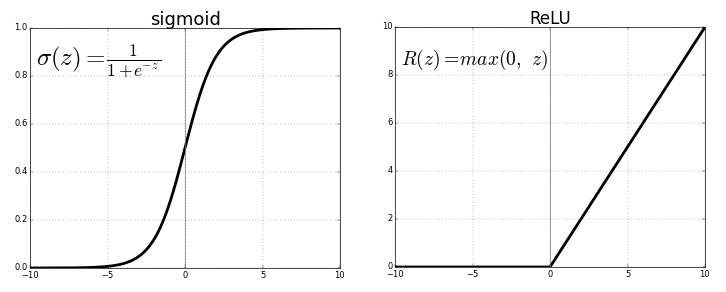
\includegraphics[scale=0.5]{sigmoid_relu}
  \caption{Sigmoid vs. ReLU}
  \label{fig:sigmoid_relu}
\end{figure}

\subsection{Tanh Layer}

The hyperbolic tangent function $tanh$ is another widely used activation function.

\begin{equation} \label{eq:tanh}
  \begin{split}
    y & = \frac{\exp{x} - \exp{-x}}{\exp{x} + \exp{-x}} \\
      & = \frac{\exp{2x} - 1}{\exp{2x} + 1} \\
      & = \frac{1- \exp{-2x}}{1 - \exp{-2x}}
  \end{split}
\end{equation}

\begin{figure}[h]
  \centering
  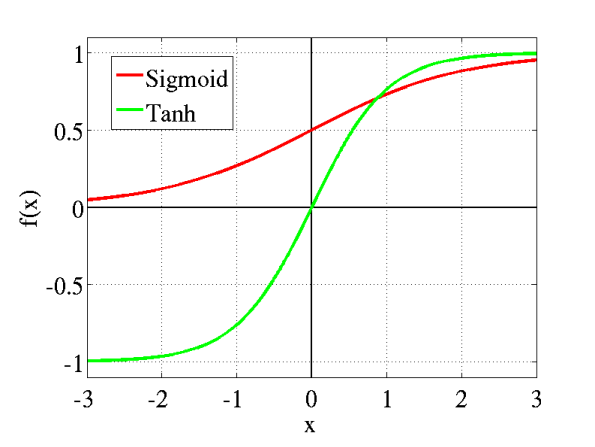
\includegraphics[scale=0.5]{sigmoid_tanh}
  \caption{Sigmoid vs. Tanh}
  \label{fig:sigmoid_tanh}
\end{figure}

\clearpage %force the next chapter to start on a new page. Keep that as the last line of your chapter!
